\chapter{Ingesters}

Ingesters are programs which collect entries from some data source and
send them to one or more indexers.

\section{Configuration}
\label{sec:global-config}

Each ingester uses its own configuration file, typically stored in
\code{/opt/gravwell/etc/}. The config file consists of two sections:

\begin{itemize}
\item
  A \code{[Global]} section, containing configuration options that
  apply to the ingester in general.
\item
  One or more named data sources which describe:
	\begin{itemize}
	\item Where to get data
	\item How to process that data into entries
	\end{itemize}
\end{itemize}

Here is a sample configuration as used by the packet capture ingester:

\begin{Verbatim}[breaklines=true]
[Global]
Ingest-Secret = IngestSecrets
Pipe-Backend-target=/opt/gravwell/comms/pipe
Log-Level=INFO #options are OFF INFO WARN ERROR
Ingest-Cache-Path=/opt/gravwell/cache/network_capture.cache

[Sniffer "spy1"]
    Interface="p1p1" #sniffing from interface p1p1
    Tag-Name="pcap"
    Snap-Len=0xffff  #maximum capture size
    BPF-Filter="not port 4023"
    Promisc=true
\end{Verbatim}

Note that it specifies the \code{[Global]} section and a single
\code{[Sniffer]} section. The \code{[Sniffer]} section describes where to get
data (from interface p1p1), which tag to apply to the entries, and some
other options. The \code{[Global]} section mostly describes how the
ingester should connect to an ingester (in this case via Unix pipe) and
how to authenticate, but it also sets up a cache and defines the level
of logging to output.

The following global configuration options are supported by all
ingesters:

\begin{itemize}
\item
  \code{Ingest-Secret}: the shared secret used to authenticate to an
  indexer. Must match indexer's Ingest-Auth setting.
\item
  \code{Insecure-Skip-TLS-Verify}: If set to true, self-signed or otherwise
  invalid TLS certificates sent by an indexer will be accepted.
\item
  \code{Ingest-Cache-Path}: A file which will be used to cache data in case
  of a network error
\item
  \code{Max-Ingest-Cache}: Maximum amount of data to cache in MB
\item
  \code{Log-Level}: A string log level. OFF, INFO, WARN, and ERROR are
  valid selections.
\item
  \code{Log-File}: The location to which logs should be written
\item
  \code{Source-Override}: An IP address (ipv4 or ipv6) which should be put
  into the ``Source'' field of entries from this ingester.
\end{itemize}

NOTE: The \code{Ingest-Secret} field \code{must} be set, but all other options
can be left blank; the defaults are sensible.

The Global section of the Ingester configuration file must also specify
at least one way to connect to an indexer. Ingesters can communicate
with an indexer in several ways:

\begin{itemize}
\item
  \textbf{Unix pipes}: Gravwell indexers typically put a Unix pipe file at
  \code{/opt/gravwell/comms/pipe}. Ingesters on the same system can connect
  to the pipe for better performance.
	\begin{itemize}
	\item \code{Pipe-Backend-target=/opt/gravwell/comms/pipe}
	\end{itemize}
\item
  \textbf{Cleartext TCP}: Gravwell indexers can accept unencrypted ingester traffic, typically
  on port 4023. This should only be used on trusted, internal networks.
	\begin{itemize}
	\item \code{Cleartext-Backend-target=127.0.0.1:4023}
	\end{itemize}
\item
  \textbf{Encrypted TCP}: Gravwell indexers, if configured with an X509 certificate/key pair,
  can accept incoming encrypted connections from ingesters. This is the
  most secure option.
	\begin{itemize}
	\item \code{Encrypted-Backend-target=127.1.1.1:4023}
	\end{itemize}
\end{itemize}

The non-Global configuration options, which define data sources, are
unique to each ingester and are described in the individual ingester
sections of this document.

\subsection{Timestamp Format Overrides (Optional)}

Data values may contain multiple timestamps, which can cause some
confusion when attempting to derive timestamps out of the data.
Normally, the Listeners will grab the left most timestamp that can be
derived, but it may be desirable to only look for a timestamp in a very
specific format. Many ingesters support the ability to specify the
exact timestamp format that the ingester via the
\code{Timestamp-Format-Override} parameter. Many timestamp
formats are available such as AnsiC, Unix, Ruby, RFC822, RFC822Z,
RFC3339, RFC3339Nano, etc. Visit the ingester documentation page for a
full list\footnote{https://docs.gravwell.io/\#!ingesters/ingesters.md}.

To force the Listener to only look for timestamps that match the
RFC3339 specification add \code{Timestamp-Format-Override=RFC3339} to the
Listener config.

\section{Simple Relay Ingester}

Simple Relay is the go-to ingester for text based data sources that can
be delivered over plaintext TCP and/or UDP network connections via
either IPv4 or IPv6.

Some common use cases for Simple Relay are:

\begin{itemize}
\item
  Remote syslog collection
\item
  Devop log collection over a network
\item
  Bro sensor log collection
\item
  Simple integration with any text source capable of delivering over a
  network
\end{itemize}

Simple Relay can ingest data in three different formats, treating each
one slightly differently:

\begin{itemize}
\item
  Line-delimited text: each line becomes one entry
\item
  RFC5424/RFC3164 syslog: each syslog message is one entry
\item
  JSON: each JSON entity becomes an entry, with the option to change
  the tag based on the value of a particular field
\end{itemize}

The Simple Relay ingester uses the unified global configuration block
described earlier. Like most other Gravwell ingesters, Simple Relay
supports multiple upstream indexers, TLS, cleartext, and named pipe
connections, a local cache, and local logging.

Simple Relay's config file specifies Listener blocks to describe how it
can accept incoming data. Listeners support several configuration
parameters for specifying protocols, listening interfaces and ports, and
fine tuning ingest behavior.

The following is a sample configuration showing all three listener types:

\begin{Verbatim}[breaklines=true]
[Global]
Ingest-Secret = IngestSecrets
Connection-Timeout = 0
Insecure-Skip-TLS-Verify=false
Cleartext-Backend-target=127.0.0.1:4023 #example of a cleartext connection
Cleartext-Backend-target=127.1.0.1:4023 #example of second cleartext connection
Encrypted-Backend-target=127.1.1.1:4024 #example of encrypted connection
Pipe-Backend-Target=/opt/gravwell/comms/pipe #a named pipe connection
Ingest-Cache-Path=/opt/gravwell/cache/simple_relay.cache #local storage cache when uplinks fail
Max-Ingest-Cache=1024 #Number of MB to store, localcache will only store 1GB before stopping
Log-Level=INFO
Log-File=/opt/gravwell/log/simple_relay.log

[Listener "default"]
    Bind-String="0.0.0.0:7777" 

[Listener "syslogtcp"]
    Bind-String="tcp://0.0.0.0:601" #standard RFC5424 reliable syslog
    Reader-Type=rfc5424
    Tag-Name=syslog
    Assume-Local-Timezone=true
    Keep-Priority=true

[JSONListener "loglistener"]
    Extractor:"user.country"
    Tag-Match="Japan":users_jp
    Tag-Match="USA":users_usa
    Default-Tag=users_other
\end{Verbatim}

\subsection{Listener Types}

As mentioned above, Simple Relay supports three different kinds of
listeners: line-delimited, syslog, and JSON. 

\subsubsection*{Line-Delimited Listeners}

Line-delimited listeners are defined with a \code{[Listener
"listener-name"]} header block as shown in the sample above. They
do not need to specify \code{Reader-Type}, since line-delimited is the
default.

A line-delimited listener will generate a new entry for every time it
sees a newline in the stream. The \code{Tag-Name} parameter can be used to
define which tag should be applied to entries; if unspecified,
``default'' will be used.

The \code{Bind-String} parameter specifies an IP and port on which
the collector should listen for incoming flow records. By default, TCP is used.
To use UDP instead, add \code{udp://}, e.g. \code{udp://0.0.0.0:514}.
Specifying an IP of 0.0.0.0 will listen on all available IP addresses.

\subsubsection*{Syslog Listeners}

RFC5424 Syslog listeners are defined with\code{[Listener
"listener-name"]} header block. The \code{Reader-Type} option must be
set to \code{rfc5424}.

To enable a listener that expects syslog messages using a reliable TCP
connection on port 601:

\begin{Verbatim}[breaklines=true]
[Listener "syslog"]
    Bind-String=0.0.0.0:601
    Reader-Type=RFC5424
\end{Verbatim}

To accept syslog messages over stateless UDP via port 514:

\begin{Verbatim}[breaklines=true]
[Listener "syslog"]
    Bind-String=udp://0.0.0.0:514
    Reader-Type=RFC524
\end{Verbatim}

RFC5424 reader types also support a parameter named
\code{Keep-Priority} which is set to true by default. A typical syslog
message is prepended by a priority identifier, however some users may
wish to discard the priority from stored messages. This is accomplished
by added \code{Keep-Priority=false} to an RFC5424 listener. Line-based listeners ignore the \code{Keep-Priority} parameter.

An example syslog message with a priority attached:

\begin{Verbatim}[breaklines=true]
<30>Sep 11 17:04:14 router dhcpd[9987]: DHCPREQUEST for 10.10.10.82 from e8:c7:4f:04:e1:af (Chromecast) via insecure
\end{Verbatim}

An example listener specification which removes the priority tag from
entries:

\begin{Verbatim}[breaklines=true]
[Listener "syslog"]
    Bind-String=udp://0.0.0.0:514
    Reader-Type=RFC524
    Keep-Priority=false
\end{Verbatim}

The \code{Tag-Name} parameter can be used to define which tag should be
applied to entries; if unspecified, ``default'' will be used.

The \code{Bind-String} parameter specifies an IP and port on which
the collector should listen for incoming flow records. By default, TCP is used.
To use UDP instead, add \code{udp://}, e.g. \code{udp://0.0.0.0:514}.
Specifying an IP of 0.0.0.0 will listen on all available IP addresses.

\subsubsection*{JSON Listeners}

The JSON Listener type enables some mild JSON processing at the time of
ingest, allowing it to apply a unique tag to an entry based on the value
of a field in a JSON entry. For instance, it may be useful to send
entries to different tags based on a ``country'' field \emph{in the JSON},
as in the following sample:

\begin{Verbatim}[breaklines=true]
{ "user": {"name":"Taka", "country":"Japan"}, "ip": "8.83.94.200" }
\end{Verbatim}

The JSON Listener requires some unique configuration options:

\begin{itemize}
\item
  \code{Extractor}: specifies the JSON extraction string, for example
  ``user.country''.
\item
  \code{Tag-Match}: specifies which tag should be applied for a given value
  extracted by the \code{Extractor}
\item
  \code{Default-Tag}: specifies the tag to use when no \code{Tag-Match} is
  applicable
\end{itemize}

Given the example JSON shown above, one possible configuration is shown
below:

\begin{Verbatim}[breaklines=true]
[JSONListener "loglistener"]
    Extractor:"user.country"
    Tag-Match="Japan":users_jp
    Tag-Match="USA":users_usa
    Default-Tag=users_other
\end{Verbatim}

This configuration will example the ``user'' element for a sub-element
named ``country''. It will compare the value of the ``country''
element to the two Tag-Match values ``Japan'' and ``USA''; if there is a
match, it will tag the entry \code{users\_jp} or \code{users\_usa},
respectively. If there is no match, the entry will be tagged
\code{users\_other}.

The \code{Bind-String} parameter specifies an IP and port on which
the collector should listen for incoming flow records. By default, TCP is used.
To use UDP instead, add \code{udp://}, e.g. \code{udp://0.0.0.0:514}.
Specifying an IP of 0.0.0.0 will listen on all available IP addresses.

\subsection{Non-Listener-Specific Configuration Options}

The configuration options in this section can be set on any type of
Listener.

\subsubsection*{Bind-String}

The \code{Bind-String} parameter controls which interface and port the
listener will bind to. The listener can bind to TCP or UDP ports,
specific addresses, and specific ports. IPv4 and IPv6 are supported.

\begin{Verbatim}[breaklines=true]
#bind to all interfaces on TCP port 7777
Bind-String=0.0.0.0:7777

#bind to all interfaces on UDP port 514
Bind-String=udp://0.0.0.0:514

#bind to port 1234 on link local IPv6 address on interface p1p
Bind-String=[fe80::4ecc:6aff:fef9:48a3%p1p1]:1234

#bind to IPv6 globally routable address on TCP port 901
Bind-String=[2600:1f18:63ef:e802:355f:aede:dbba:2c03]:901
\end{Verbatim}

\subsubsection*{Ignore-Timestamps (Optional)}

The \code{Ignore-Timestamps} parameter instructs the listener to apply the
current timestamp to entries rather than attempting to extract a
timestamp from them. This parameter is useful when reading data where
there may not be a timestamp present, or the timestamp is wrong on the
originating system due to unreliable system clocks.
\code{Ignore-Timestamps} is false by default.

\subsubsection{Assume-Local-Timezone (Optional) and Timezone-Override (Optional)}

Most timestamp formats have a timezone attached which indicates an
offset to Universal Coordinated Time (UTC). However, some systems do not
specify the timezone, leaving it up to the receiver to determine what
timezone a log entry may be in. \code{Assume-Local-Timezone} makes the
Listener assume that the timestamp is in the same timezone as the Simple
Relay reader when the timezone is omitted. \code{Timezone-Override} takes a
string in the IANA timezone database format (e.g. "America/Chicago") and
applies that timezone to timestamps which do not specify a timezone.

\code{Assume-Local-Timezone} and \code{Timezone-Override} are mutually
exclusive.

\subsubsection*{Source-Override (Optional)}

The \code{Source-Override} parameter instructs the Listener to ignore the
source of the data and apply a hard coded value. It may be desirable to
hard-code source values for incoming data as a method to organize and/or
group data sources. \code{Source-Override} values can be IPv4 or IPv6
values.

\begin{Verbatim}[breaklines=true]
Source-Override=192.168.1.1
Source-Override=127.0.0.1
Source-Override=[fe80::899:b3ff:feb7:2dc6]
\end{Verbatim}

\subsection{Hands-On Lab: Simple Relay}

In this lab we will stand up a Simple Relay ingester and send some
traffic to it manually using netcat. First, launch a Gravwell
webserver+indexer container:

\begin{Verbatim}[breaklines=true]
docker run --rm --net gravnet -p 8080:80 -d --name gravwell gravwell:base
\end{Verbatim}

Open the web interface by pointing your browser at \href{http://localhost:8080/}{http://localhost:8080} and log in (``admin''/``changeme''). Then start the ingester container running the Simple Relay ingester:

\begin{Verbatim}[breaklines=true]
docker run --rm --net gravnet --name ingesters -it \
-e GRAVWELL_CLEARTEXT_TARGETS=gravwell:4023 \
gravwell:ingesters /opt/gravwell/bin/gravwell_simple_relay
\end{Verbatim}

Note the use of the option \code{-e GRAVWELL\_CLEARTEXT\_TARGETS=gravwell:4023}.
This sets an environment
variable within the container that tells the ingester which indexer it
should connect to.

The ingesters container ships with a default Simple Relay configuration
which listens for line-delimited entries on port 7777, shown below:

\begin{Verbatim}[breaklines=true]
[Global]
Log-Level=INFO

[Listener "default"]
    Bind-String="0.0.0.0:7777"
    Ignore-Timestamps=true
    Tag-Name=default
\end{Verbatim}

Note that this configuration does not define an ingest authentication
secret or any indexer connection information. These are instead passed
as environment variables to the Docker container.

We'll stand up a third container in order to send some entries by
hand:

\begin{Verbatim}[breaklines=true]
docker run --net gravnet -it busybox /bin/sh
\end{Verbatim}

{From the shell prompt, we can run netcat and hand-type some entries (in
this case ``foo'' and ``bar''), then hit Ctrl-C when done:}

\begin{Verbatim}[breaklines=true]
nc ingesters 7777
foo
bar
\end{Verbatim}

We can verify that the entries have been ingested by running the search
\code{tag=default} as shown in Figure \ref{fig:simple-relay-lab}.

\begin{figure}
	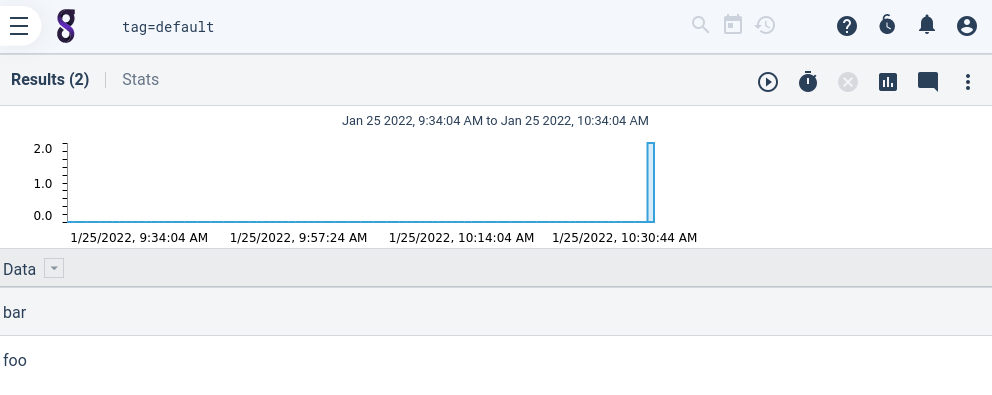
\includegraphics{images/igst-syslog-lab.png}
	\caption{Entries from Simple Relay Ingester}
	\label{fig:simple-relay-lab}
\end{figure}

To clean up after the experiment, simply run:

\code{docker kill \$(docker ps -a -q)}

\subsubsection{Lab Questions}

\begin{enumerate}
\item
  How would you convert the listener to a syslog listener?
\item
  How would you make the Listener listen for incoming UDP rather than
  TCP?
\end{enumerate}

\section{File Follower Ingester}

The File Follower ingester is the best way to ingest files on the local
filesystem in situations where those files may be updated on the fly. It
ingests each line of the files as a single entry.

The most common use case for File Follower is monitoring a directory
containing log files which are actively being updated, such
as \code{/var/log}. It intelligently handles log rotation, detecting when
\code{logfile} has been moved to \code{logfile.1} and so on. It can be configured to
ingest files matching a specific pattern in a directory, optionally
recursively descending into the subdirectories of that top-level
directory.

The File Follower ingester uses the unified global configuration block
described in Section \ref{sec:global-config}. Like most other Gravwell ingesters,
File Follower supports multiple upstream indexers, TLS, cleartext, and
named pipe connections, and local logging.

Below is an example configuration for the File Follower ingester,
configured to watch several different types of log files in
\code{/var/log} and recursively follow files under \code{/tmp/incoming}:

\begin{Verbatim}[breaklines=true]
[Global]
Ingest-Secret = IngestSecrets
Insecure-Skip-TLS-Verify = false
Cleartext-Backend-target=172.20.0.1:4023
Cleartext-Backend-target=172.20.0.2:4023
State-Store-Location=/opt/gravwell/etc/file_follow.state
Log-Level=ERROR
Max-Files-Watched=64

[Follower "syslog"]
        Base-Directory="/var/log/"
        File-Filter="syslog,syslog.[0-9]" 
        Tag-Name=syslog
        Assume-Local-Timezone=true
[Follower "external"]
        Base-Directory="/tmp/incoming"
        Recursive=true
        File-Filter="*.log"
        Tag-Name=external
        Timezone-Override="America/Los_Angeles"
\end{Verbatim}

In this example, the syslog follower reads \code{/var/log/syslog} and
its rotations, ingesting lines to the syslog tag and assuming dates to
be in the local timezone. The external follower reads all files ending
in .log from the directory \code{/tmp/incoming}, descending recursively
into directories. It parses timestamps as though they were in the
Pacific time zone. This follower illustrates a configuration that would
be useful if, for example, several servers on the US west coast
periodically uploaded their log files to this system.

The configuration parameters used above are explained in greater detail
in the following sections.

\subsection{Additional Global Parameters}

The File Follower ingester defines several additional parameters for
the \code{[Global]} section. These parameters apply to \emph{all} Followers
defined in the config file.

\subsubsection{Max-Files-Watched}

The \code{Max-Files-Watched} parameter prevents the File Follower from
maintaining too many open file descriptors. If
\code{Max-Files-Watched=64} is specified, the File Follower will actively
watch up to 64 log files. When a new file is created, the File Follower
will stop actively watching the oldest existing file in order to watch
the new one. However, if the old file is later updated, it will return
to the top of the queue.

We recommend leaving this setting at 64 in most cases; configuring the
limit too high can run into limits set by the kernel.

\subsection{Follower Configuration Parameters}

The File Follower configuration file contains one or more ``Follower''
directives:

\begin{Verbatim}[breaklines=true]
[Follower "syslog"]
        Base-Directory="/var/log/"
        File-Filter="syslog,syslog.[0-9]"
        Tag-Name=syslog
\end{Verbatim}

Each follower specifies at minimum a base directory and a filename
filtering pattern. This section describes possible configuration
parameters which can be set per follower.

\subsubsection{Base-Directory}

The \code{Base-Directory} parameter specifies the directory which will
contain the files to be ingested. It should be an absolute path and
contain no wildcards.

\subsubsection{File-Filter}

The \code{File-Filter} parameter defines the filenames which should be
ingested. It can be as simple as a single file name:

\code{File-Filter="foo.log"}

Or it can contain multiple patterns:

\code{File-Filter="kern*.log,kern*.log.{[}0-9{]}"}

which will match any filenames beginning with ``kern'' and ending with
``.log'', or beginning with ``kern'' and ending with ``.log.0''
through ``.log.9''.

The full matching syntax, as defined
in \href{https://golang.org/pkg/path/filepath/\#Match}{https://golang.org/pkg/path/filepath/\#Match}, is:

\begin{Verbatim}[breaklines=true]
pattern:
    { term }
term:
    '*'         matches any sequence of non-Separator characters
    '?'         matches any single non-Separator character
    '[' [ '^' ] { character-range } ']'
                character class (must be non-empty)
    c           matches character c (c != '*', '?', '\\', '[')
    '\\' c      matches character c

character-range:
    c           matches character c (c != '\\', '-', ']')
    '\\' c      matches character c
    lo '-' hi   matches character c for lo <= c <= hi
\end{Verbatim}

\subsubsection{Tag-Name (Optional)}

The \code{Tag-Name} parameter specifies the tag to apply to entries
ingested by this follower. If unset, the ``default'' tag is used.

\subsubsection{Ignore-Timestamps (Optional)}

The \code{Ignore-Timestamps} parameter indicates that the follower should
not attempt to extract a timestamp from each line of the file, but
rather tag each line with the current time.

\subsubsection{Assume-Local-Timezone (Optional)}

\code{Assume-Local-Timezone} is a boolean setting which directs the ingester
to parse timestamps which lack timezone specifications as though they
were in the local time zone rather than the default UTC.

\code{Assume-Local-Timezone} and \code{Timezone-Override} are mutually
exclusive.

\subsubsection{Timezone-Override (Optional)}

The \code{Timezone-Override} parameter directs the ingester to parse
timestamps which lack timezone specifications as though they were in the
given time zone rather than the default UTC.

The timezone should be specified in IANA database string format as
defined at \href{https://en.wikipedia.org/wiki/List\_of\_tz\_database\_time\_zones}{https://en.wikipedia.org/wiki/List\_of\_tz\_database\_time\_zones};
for example, US Central Time should be specified as follows:

\code{Timezone-Override="America/Chicago"}

\code{Assume-Local-Timezone} and \code{Timezone-Override} are mutually
exclusive.

\code{Timezone-Override="Local"} is functionally equivalent to
\code{Assume-Local-Timezone=true}

\subsubsection{Recursive (Optional)}

The \code{Recursive} parameter directs the File Follower to ingest all
files matching the \code{File-Filter} \emph{recursively} under the
\code{Base-Directory}.

By default, the ingester will only ingest those files matching the
\code{File-Filter} under the top level of the \code{Base-Directory}; the
following would ingest \code{/tmp/incoming/foo.log} but not
\code{/tmp/incoming/system1/foo.log}:

\begin{Verbatim}[breaklines=true]
Base-Directory="/tmp/incoming"
File-Filter="foo.log"
\end{Verbatim}

By setting \code{Recursive=true}, the configuration will ingest
\emph{any} file named \code{foo.log} at any directory depth under
\code{/tmp/incoming}.

\subsubsection{Ignore-Line-Prefix (Optional)}

The ingester will drop (not ingest) any lines beginning with the string
passed to \code{Ignore-Line-Prefix}. This is useful when ingesting log
files which contain comments, such as Bro logs. The
\code{Ignore-Line-Prefix} parameter may be specified multiple times. The
following indicates that lines beginning with \# or // should not be
ingested:

\begin{Verbatim}[breaklines=true]
Ignore-Line-Prefix="#"
Ignore-Line-Prefix="//"
\end{Verbatim}

Each follower can specify a unique timestamp format using the
\code{Timestamp-Format-Override} parameter.

\subsubsection{Timestamp-Delimited (Optional)}

The \code{Timestamp-Delimited} parameter is a boolean specifying that each
occurrence of a time stamp should be considered the start of a new
entry. This is useful when log entries may span multiple lines. When
specifying \code{Timestamp-Delimited}, the
\code{Timestamp-Format-Override} parameter must also be set. Let's look at
a file snippet and explore how timestamp delimiting would affect entry
extraction. If we assume the following snippet:

\begin{Verbatim}[breaklines=true]
2012-11-01T22:08:41+00:00 Line 1 of the first entry
Line 2 of the first entry
2012-11-01T22:08:43+00:00 Line 1 of the second entry
Line 2 of the second entry
\end{Verbatim}

The entries extracted would be:

\textbf{Entry 1:}

\begin{Verbatim}[breaklines=true]
2012-11-01T22:08:41+00:00 Line 1 of the first entry
Line 2 of the first entry
\end{Verbatim}

\textbf{Entry 2:}

\begin{Verbatim}[breaklines=true]
2012-11-01T22:08:43+00:00 Line 1 of the second entry
Line 2 of the second entry
\end{Verbatim}

\subsection{Hands-On Lab: File Follower}

In this lab, we will use the File Follower to ingest Linux system logs.
First, launch a Gravwell webserver+indexer container:

\begin{Verbatim}[breaklines=true]
docker run --rm --net gravnet -p 8080:80 -d \
--name gravwell gravwell:base
\end{Verbatim}

Next, we create the ingester container. It needs some additional
configuration, so we use \code{docker create} rather than \code{docker start}:

\begin{Verbatim}[breaklines=true]
docker create --rm --net gravnet --name ingesters -it -e \
GRAVWELL_CLEARTEXT_TARGETS=gravwell:4023 -v /var/log:/var/log \
gravwell:ingesters /opt/gravwell/bin/gravwell_file_follow -v
\end{Verbatim}

Note the option \code{-v /var/log:/var/log}. This mounts the host's
log directory into the container. In this lab, we will be ingesting the
\emph{host's} logs, since Docker containers do not generate many log
files.

The File Follower in the container is pre-configured with these
Follower definitions:

\begin{Verbatim}[breaklines=true]
[Follower "auth"]
    Base-Directory="/var/log/"
    File-Filter="auth.log,auth.log.[0-9]"
    Tag-Name=auth
[Follower "kernel"]
    Base-Directory="/var/log"
    File-Filter="dmesg,dmesg.[0-9]"
    Tag-Name=kernel
[Follower "kernel2"]
    Base-Directory="/var/log"
    File-Filter="kern.log,kern.log.[0-9]"
    Tag-Name=kernel
\end{Verbatim}

There is a problem with the configuration as it stands. Linux log
timestamps don't include a time zone, and your system is probably set to
the local time zone, so the log files will contain entries with local
timestamps. Docker containers default to UTC, though, so the ingester
will improperly parse the log timestamps. Luckily, this can be fixed in
the config file. 

\textbf{NOTE:} If your host computer is set to UTC, you can skip these config modifications and skip straight to starting the ingester.

We'll first copy out the config file from the ingester:

\begin{Verbatim}[breaklines=true]
docker cp ingesters:/opt/gravwell/etc/file_follow.conf /tmp
\end{Verbatim}

Edit the file and add the following to each
\code{Follower}block, substituting your timezone:

\code{Timezone-Override="America/Denver"}

And push the configuration back to the ingester:

\begin{Verbatim}[breaklines=true]
docker cp /tmp/file_follow.conf ingesters:/opt/gravwell/etc/file_follow.conf 
\end{Verbatim}

With the configuration fixed, we can start the ingester:

\begin{Verbatim}[breaklines=true]
docker start ingesters
\end{Verbatim}

Recall that we passed the -v flag to \code{gravwell\_file\_follow}
when we created the container; this enables verbose mode, which allows us to see every entry
the ingester reads \emph{and} the timestamp it derived from the log entry.
Most ingesters support the -v flag. You can view the log output by running
the command \code{docker log ingesters}; the following is a sample:

\code{GOT 2019-03-09T13:12:59-07:00 Mar ~9 13:12:59 bombadil kernel:
{[}7955880.007543{]} hub 2-1:1.0: 3 ports detected}

The portion \code{GOT 2019-03-09T13:12:59-07:00} indicates that the
ingester has parsed out a timestamp of March 9, 13:12:59 US Mountain
Time from the log entry, which comprises the rest of the line.

Based on the configuration, we can expect to see entries tagged
``auth'' and ``kernel'', and a quick search for \code{tag=auth} should
confirm this, as shown in Figure \ref{fig:file-follow-lab}.

\begin{figure}
	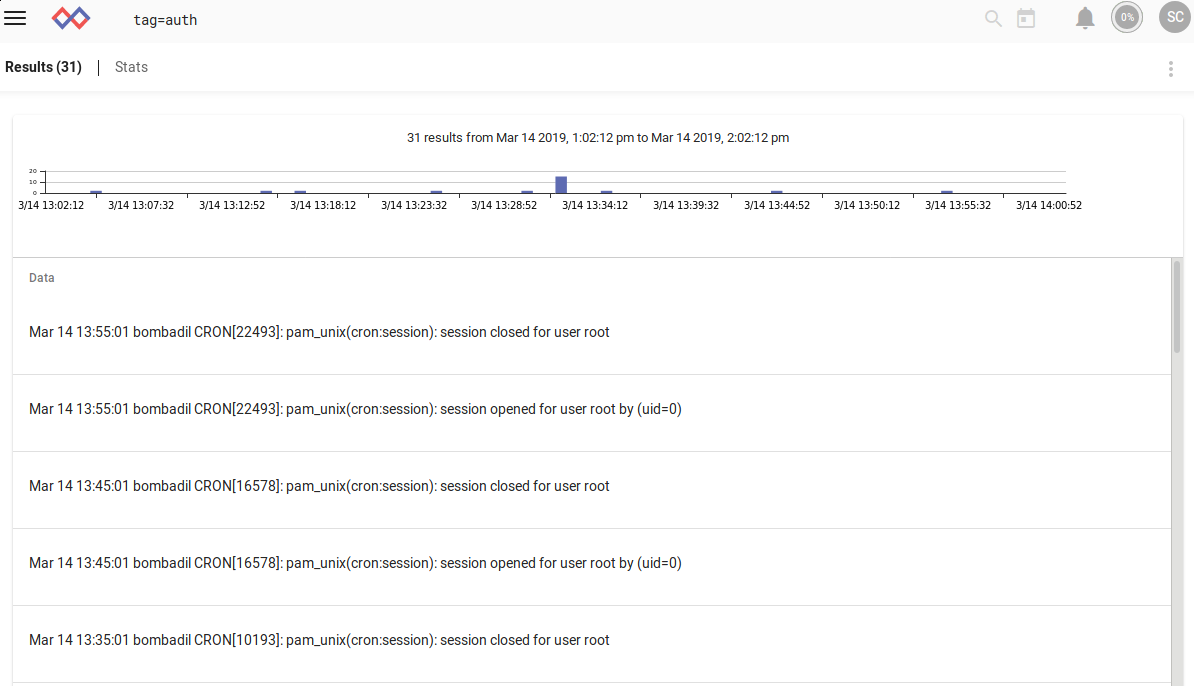
\includegraphics{images/igst-filefollow-lab.png}
	\caption{Ingested Logs}
	\label{fig:file-follow-lab}
\end{figure}

To clean up after the experiment, simply run:

\code{docker kill \$(docker ps -a -q)}

\subsubsection{Lab Questions}

\begin{enumerate}
\item
  Suppose we wanted to ingest \emph{all} files ending in \code{.log} in
  \code{/var/log}, including files in subdirectories. Configure a Follower that
  would accomplish this.
\end{enumerate}

%%%%%%%%%%%%%%%%%%%%%%%%%%%%%%%%%%%%%%%%%%%%%%%%%%%%%%%%%%%%
% TODO: this section is completely different from the others and as much of a tutorial
% about the winlog module as the ingester itself
%%%%%%%%%%%%%%%%%%%%%%%%%%%%%%%%%%%%%%%%%%%%%%%%%%%%%%%%%%%%
\section{Windows Event Ingester}

The Windows event ingester is designed to monitor the Windows event
service and ingest raw events into Gravwell. Windows events are
formatted in XML and frankly, can get a little unruly; as a result the
Windows ingester supports the ability to subscribe to specific event
streams and filter based on Provider and EventID directly in the
ingester. While Gravwell is typically an ``ingest first and ask
questions later'' kind of company, the Windows logging system produces a
tremendous amount of un-useful events that are large and complex to
parse. If you are monitoring significant Windows infrastructure, it may
not be necessary to ingest 100GB of XML that tells you every time a
desktop goes to sleep or wakes up.

The Windows event ingester is a system service and is installed into
\code{\%ProgramFiles\%\textbackslash{}gravwell}. The service is configured
via a \code{config.cfg} file located in the same directory. Configuration
is similar to other ingesters and shares the common
\code{[Global]} block which defines how the ingester will authenticate
and communicate with indexers. After the \code{[Global]} section, the config
file can define subscriptions for Windows event channels. Each EventChannel can
specify a tag, maximum reachback, and filters for the provider, event
id, and level. Available configuration parameters for an EventChannel
are as follows:

\begin{itemize}
\item \code{Tag-Name}: Specifies the tag the events will go to.
\item \code{Provider}: Filter to control which providers the ingester will send to indexers.
\item \code{EventID}: Controls which event IDs are sent to indexers.
\item \code{Level}: Controls minimum alert level.
\item \code{Max-Reachback}: Controls a maximum age of entries the ingester will read on first start.
\end{itemize}

For example, let's look at an event channel configuration which
subscribes to the ``security'' channel:

\begin{Verbatim}[breaklines=true]
[EventChannel "security"]
    Tag-Name=windows
    Channel=Security
\end{Verbatim}

This configuration specifies that the ingester should send all events
on the security channel to the tag windows. Because we haven't
specified any filters or a \code{Max-Reachback}, the ingester will grab all
historical events that are available from the \code{Security} channel and
send every one of them to the indexer. It then begins streaming new
events as they come in.

Let's next examine a configuration that applies some
filters to control what we ingest:

\begin{Verbatim}[breaklines=true]
[EventChannel "sysmon"]
    Tag-Name=sysmon
    Channel=Microsoft-Windows-Sysmon/Operational
    Max-Reachback=24h
    Level=4
    EventID=4000-5000
\end{Verbatim}

This configuration reads entries from the
\code{Microsoft-Windows-Sysmon/Operational} channel, but only if the Level
is 4 and the EventID is between 4000 and 5000. When the Ingester first
starts it will also retrieve entries from the Windows event store that
are up to 24 hours old. Tailoring the configuration can help narrow in
on event sources and event IDs that actually have relevance to your
mission, whether it be compliance, security, or performance monitoring.

Let's take a look at a windows log entry that has been formatted so
that we can see some of its structure:

\begin{Verbatim}[breaklines=true]
<?xml version="1.0" encoding="UTF-8"?>
<Event xmlns="http://schemas.microsoft.com/win/2004/08/events/event">
   <System>
      <Provider Name="Microsoft-Windows-Kernel-Power"
Guid="{331c3b3a-2005-44c2-ac5e-77220c37d6b4}" />
      <EventID>107</EventID>
      <Version>1</Version>
      <Level>4</Level>
      <Task>102</Task>
      <Opcode>0</Opcode>
      <Keywords>0x8000000000000444</Keywords>
      <TimeCreated SystemTime="2019-03-23T21:15:39.4065468Z"/>
      <EventRecordID>2243</EventRecordID>
      <Correlation />
      <Execution ProcessID="4" ThreadID="9996"/>
      <Channel>System</Channel>
      <Computer>rebecca-PC</Computer>
      <Security />
   </System>
   <EventData>
      <Data Name="TargetState">4</Data>
      <Data Name="EffectiveState">5</Data>
      <Data Name="WakeFromState">4</Data>
      <Data Name="WakeRequesterTypeAc">2</Data>
      <Data Name="WakeRequesterTypeDc">0</Data>
   </EventData>
</Event>
\end{Verbatim}

The log is large and unruly, there is a lot of repetition. Fortunately
the \code{winlog} search module can help simplify working with windows XML
logs. Let's start by executing a query that extracts the Provider and
EventID. We will then filter the extracted values to only look at the
\code{Microsoft-Windows-Sysmon} provider and EventID 1. The winlog
search module supports several shortcuts that can make it easier to
extract data from the Windows XML structures. The shortcuts allow us to
specify most of the system members directly by name, any other arguments
which do not specify a system field member is assumed to be a data field
member. Refer to the winlog online documentation for a full list of extractions.\footnote{https://docs.gravwell.io/\#!search/winlog/winlog.md}

For example, if we want the Provider and EventID fields, we can
execute the query \code{winlog Provider EventID}; the winlog module knows
where those fields are located within the XML document. If we wanted the data field named
``TargetState'', we can just pass the argument \code{TargetState}. The
\code{winlog} module figures out that it's not a known system field and
assumes it is a data name field. Given the example entry above, if we
executed the following query:


\code{tag=windows winlog Provider EventID WakeFromState}

The following Enumerated values would be extracted:

\begin{longtable}[]{lr}
\toprule
\endhead
\textbf{Name} & \textbf{Value} \\
{Provider} & {Microsoft-Windows-Kernel-Power} \\
{EventID} & {107} \\
{WakeFromState} & {4} \\
\bottomrule
\end{longtable}

The winlog module supports inline filtering (which is covered in depth
in later chapters), so we can pass equality statements to each argument to
filter down to specific events. For example, if we wanted to only look
at events from the \code{Microsoft-Windows-Sysmon} provider we would
execute the following query:

\code{tag=windows winlog Provider=="Microsoft-Windows-Sysmon"}

%%%%%%%%%%%%%%%%%%%%%%%%%%%%%%%%%%%%%%%%%%%%%%%%%%%%%%%%%%%%%%%%
% TODO: This lab is inappropriate for the ingesters chapter, rework it or move it
%%%%%%%%%%%%%%%%%%%%%%%%%%%%%%%%%%%%%%%%%%%%%%%%%%%%%%%%%%%%%%%%
\subsection{Hands-on Lab: Windows logs}

Windows logs are normally XML, which is a large and often complex
format. Gravwell provides the \code{winlog} search module that can help
with extracting useful data from Windows logs. For this lab we will
examine some Windows logs and extract some basic data so that we can
track process creation using
sysmon\footnote{https://docs.microsoft.com/en-us/sysinternals/downloads/sysmon} using the
SwiftOnSecurity configuration
set\footnote{https://raw.githubusercontent.com/SwiftOnSecurity/sysmon-config/master/sysmonconfig-export.xml}. For more information refer to our our Windows events documentation
page\footnote{https://docs.gravwell.io/\#!ingesters/ingesters.md\#Windows\_Event\_Service}

We can't run the Windows ingester on Docker, so instead we will just
import some Windows logs and poke around a bit. We'll fire up a test
container and push in the Windows logs using the \code{regexFile} ingester.
The regexFile ingester is a one-off ingester that can assist in
ingesting single files where the entry delimiter is more complex than a simple newline.
Windows logs often have spaces and newlines in them, so we are going to use
the regexFile ingester to break on XML boundaries. Take note of the
\code{rexp} argument; it's a regular expression that will match the
beginning of a Windows log entry.

First, we start the indexer and webserver:

\begin{Verbatim}[breaklines=true]
docker run --rm -d -p 8080:80 --net gravnet --name test gravwell:base
\end{Verbatim}

Now we'll push in some data with the reimport ingester:

\begin{Verbatim}[breaklines=true]
cd ~/gravwell_training/Ingesters/Lab-Winevent
docker run -v $PWD/data:/tmp/data --rm -i --net gravnet \
gravwell:ingesters /opt/gravwell/bin/reimport -rebase-timestamp \
-clear-conns test:4023 -i /tmp/data/winlog.json -import-format json
\end{Verbatim}

Log into the web GUI (\href{http://localhost:8080}{http://localhost:8080}) and perform the following queries:

\begin{enumerate}
\item Use the winlog search module to get all entries that represent process creation events with the following constraints:
	\begin{enumerate}
	\item Provider is \code{Microsoft-Windows-Sysmon}
	\item EventID is 1
	\end{enumerate}
\item Extract the Computer and CommandLine fields and make a table with those columns
\end{enumerate}

To clean up after the experiment, simply run:

\code{docker kill \$(docker ps -a -q)}


\subsubsection{Lab Questions:}

\begin{enumerate}
\item Do you see any command line processes that look interesting?
\item Are there any large parameters that you could decode?
	\begin{enumerate}
	\item How would you do it?
	\end{enumerate}
\end{enumerate}

\section{Netflow and IPFIX Ingester}

The Netflow ingester acts as a Netflow collector, gathering records
created by Netflow exporters and capturing them as Gravwell entries for
later analysis. These entries can then be analyzed using the netflow
search module. The Netflow ingester currently only accepts traffic via
UDP.

A sample configuration is shown below:

\begin{Verbatim}[breaklines=true]
[Global]
Ingest-Secret = IngestSecrets
Connection-Timeout = 0
Insecure-Skip-TLS-Verify=false
Pipe-Backend-target=/opt/gravwell/comms/pipe #a named pipe connection, this should be used when ingester is on the same machine as a backend
Log-Level=INFO

[Collector "netflow v5"]
    Bind-String="0.0.0.0:2055" #we are binding to all interfaces
    Tag-Name=netflow

[Collector "ipfix"]
    Tag-Name=ipfix
    Bind-String="0.0.0.0:6343"
    Flow-Type=ipfix
\end{Verbatim}

This configuration defines two collectors, one for Netflow v5, one for
IPFIX. The Netflow collector listens on UDP port 2055 and tags its
entries ``netflow'', while the IPFIX collector listens on UDP port 6343
and tags its entries ``ipfix''.

Note that the ``ipfix'' collector type can accept both IPFIX and Netflow v9 data.

\subsection{Collector Configuration Parameters}

\subsubsection{Bind-String}

The \code{Bind-String} parameter specifies an IP and UDP port on which
the collector should listen for incoming flow records. Specifying an IP
of 0.0.0.0 will listen on all available IP addresses.

\subsubsection{Tag-Name (Optional)}

The \code{Tag-Name} parameter specifies the tag to apply to entries
ingested by this follower. If not specified, the ``default'' tag is
used.

\subsubsection{Flow-Type (Optional)}

The \code{Flow-Type} parameter specifies which type of flows the collector
should read. The available options are ``netflowv5'' and ``ipfix''; the
default is ``netflowv5''.

\subsection{Hands-on Lab: Netflow Ingester}

In this lab, we will ingest procedurally-generated Netflow records.
First, launch a Gravwell webserver+indexer container:

\begin{Verbatim}[breaklines=true]
docker run --rm --net gravnet -p 8080:80 -d --name gravwell gravwell:base
\end{Verbatim}

Next, start the ingester container running the netflow ingester:

\begin{Verbatim}[breaklines=true]
docker run --rm --net gravnet --name ingesters -it \
-e GRAVWELL_CLEARTEXT_TARGETS=gravwell:4023 \
gravwell:ingesters /opt/gravwell/bin/gravwell_netflow_capture
\end{Verbatim}

The netflow ingester is pre-configured to listen on port 2055 for
incoming Netflow v5 records.

Now, we use another Docker container to generate Netflow records and
send them to the ingester:

\begin{Verbatim}[breaklines=true]
docker run -it --net gravnet --rm \
networkstatic/nflow-generator -t ingesters -p 2055
\end{Verbatim}

The netflow generator will run indefinitely, generating flow records,
until killed.

Log into the web GUI (\href{http://localhost:8080}{http://localhost:8080}).
We can now search the netflow data:

\begin{Verbatim}[breaklines=true]
tag=netflow netflow Bytes Src | stats sum(Bytes) by Src | table Src sum
\end{Verbatim}

We should see traffic originating from many (randomly-generated) IP addresses, as shown in Figure \ref{fig:netflow-lab}.

\begin{figure}
	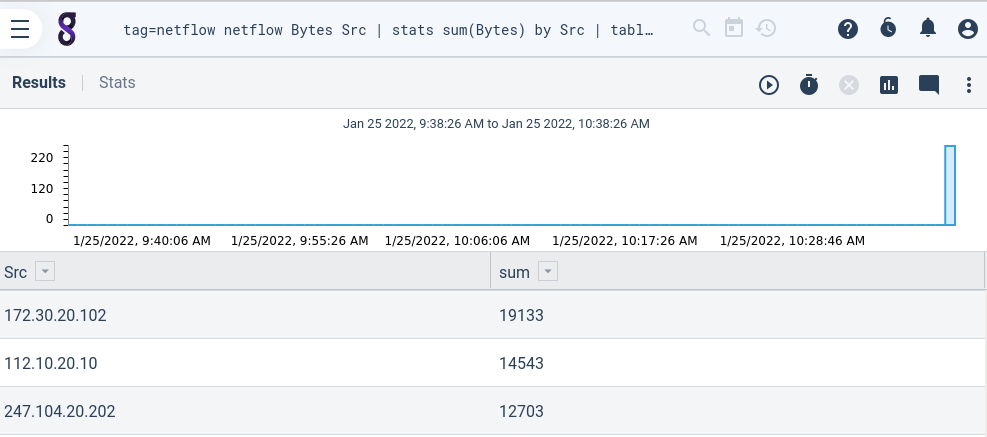
\includegraphics{images/igst-netflow-lab.png}
	\caption{Netflow Query Results}
	\label{fig:netflow-lab}
\end{figure}

To clean up after the experiment, simply run:

\code{docker kill \$(docker ps -a -q)}




\section{Packet Capture Ingester}

The packet capture ingester illustrates one of Gravwell's unique
strengths: its ability to ingest raw, unprocessed binary data. This
ingester listens on one or more network interfaces and ingests every
packet it sees in a separate entry. Later, those packets can be parsed
using the `packet' search module.

A sample configuration is shown below:

\begin{Verbatim}[breaklines=true]
[Global]
Ingest-Secret = IngestSecrets
Connection-Timeout = 100s
Cleartext-Backend-target=192.168.0.1:4023 #example of adding another cleartext connection
Max-Ingest-Cache=32
Ingest-Cache-Path=/opt/gravwell/cache/network_capture.cache

[Sniffer "spy1"]
    Interface="eth0" #sniffing from interface eth0
    Tag-Name="pcap"  #assigning tag pcap
    Snap-Len=0xffff  #maximum capture size
    BPF-Filter="not port 4023" #do not sniff any traffic on our backend connection
    Promisc=true
\end{Verbatim}

This configuration defines a single Sniffer, which listens for packets
on interface \code{eth0}, tags them as ``pcap'', and ships them to an
indexer via an unencrypted connection. Note the use of the
\code{BPF-Filter} option; this tells the ingester to ignore packets on port
4023, because the ingester is using port 4023 to transfer entries to the
indexer. If this option was not set, every entry sent to the indexer
would result in at least one additional entry being generated!

\subsection{Hands-on Lab: Packet Capture Ingester}

This lab will demonstrate ingestion of packets. First, launch a base
Gravwell container:

\begin{Verbatim}[breaklines=true]
docker run --rm --net gravnet -p 8080:80 -d --name gravwell gravwell:base
\end{Verbatim}

Log into the web GUI (\href{http://localhost:8080}{http://localhost:8080}) once the container is started.

Next, start the ingester container running the packet capture
ingester:

\begin{Verbatim}[breaklines=true]
docker run --rm --net gravnet --name pcap -d \
-e GRAVWELL_CLEARTEXT_TARGETS=gravwell:4023 \
gravwell:pcap \ /opt/gravwell/bin/gravwell_network_capture
\end{Verbatim}


The ingester is pre-configured to capture packets on the eth0
interface. The ingester should start seeing packets soon, even without
generating any traffic; this can be verified by searching for
\code{tag=pcap} as shown in Figure \ref{fig:pcap-lab1}.

\begin{figure}
	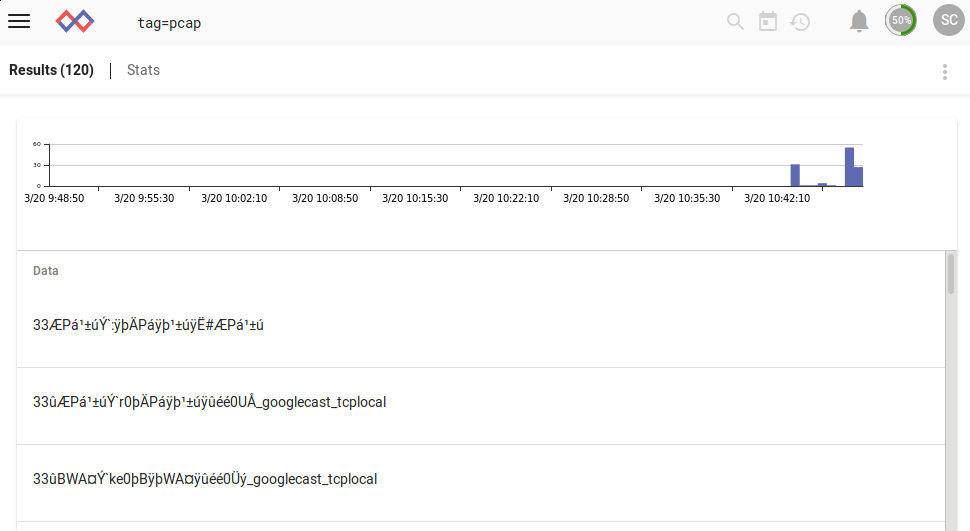
\includegraphics{images/igst-pcap-lab1.png}
	\caption{Raw packets}
	\label{fig:pcap-lab1}
\end{figure}

Note that the packets are ``garbage''. This is because the packets were
captured as binary blobs, and without specifying how to parse them,
Gravwell can only print an ASCII representation of the binary.

We can see which protocols are in use by extracting the source IP,
dest IP, and IP protocol from each packet. Results are shown in Figure \ref{fig:pcap-lab2}.

\code{tag=pcap packet ipv4.SrcIP ipv4.DstIP ipv4.Protocol \textbar{} table}


\begin{figure}
	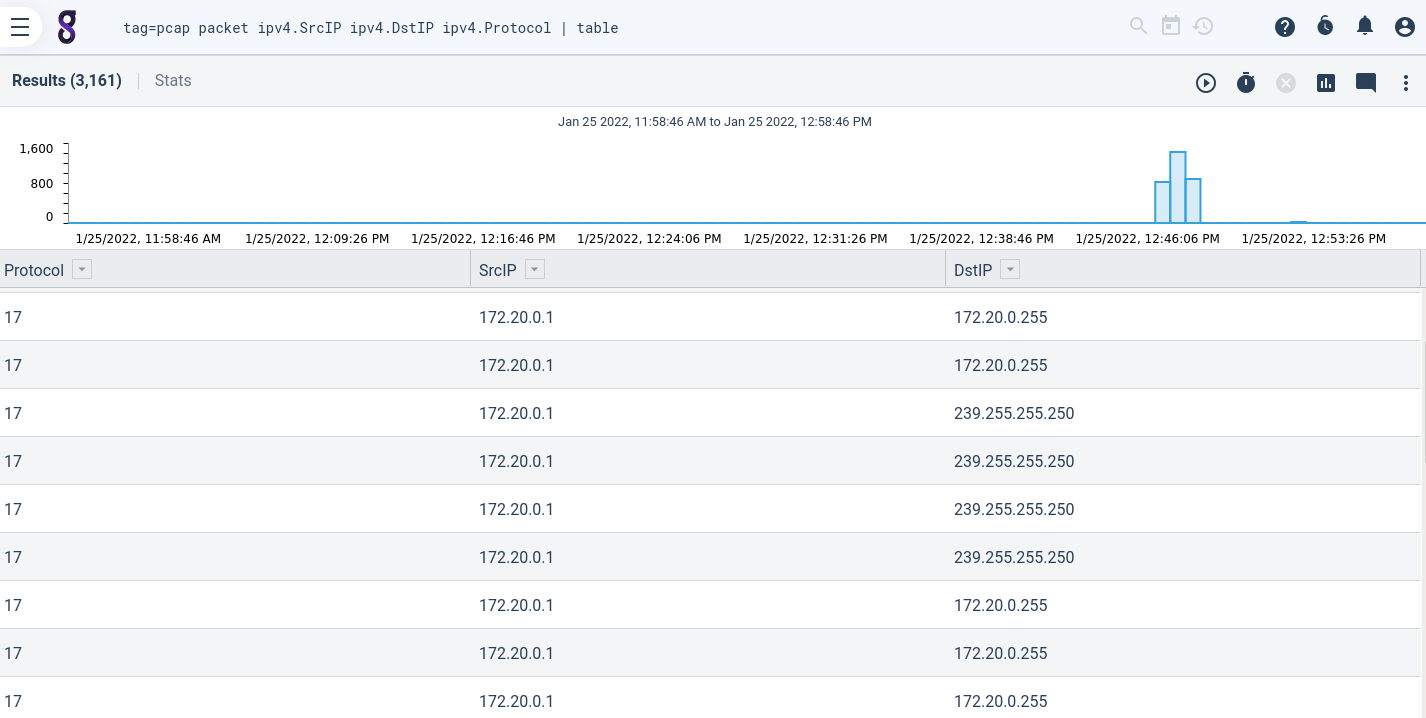
\includegraphics{images/igst-pcap-lab2.png}
	\caption{Parsing Packets}
	\label{fig:pcap-lab2}
\end{figure}

The screenshot shows that the majority of packets are currently
protocol 17 (UDP) with the occasional protocol 2 packet (IGMP).

Next, we'll generate some ping traffic:

\begin{Verbatim}[breaklines=true]
docker run -it --net gravnet --rm gravwell:base ping pcap
\end{Verbatim}

We can then run a search which limits results only to protocol 1
(ICMP):


\code{tag=pcap packet ipv4.SrcIP ipv4.DstIP ipv4.Protocol==1 \textbar{}
table}

We can see which protocol is appearing most frequently by running the
following query:

\code{tag=pcap packet ipv4.Protocol \textbar{} count by Protocol \textbar{}
chart count by Protocol}

The results are shown in Figure \ref{fig:pcap-lab3}, with the chart changed to a pie chart.

\begin{figure}
	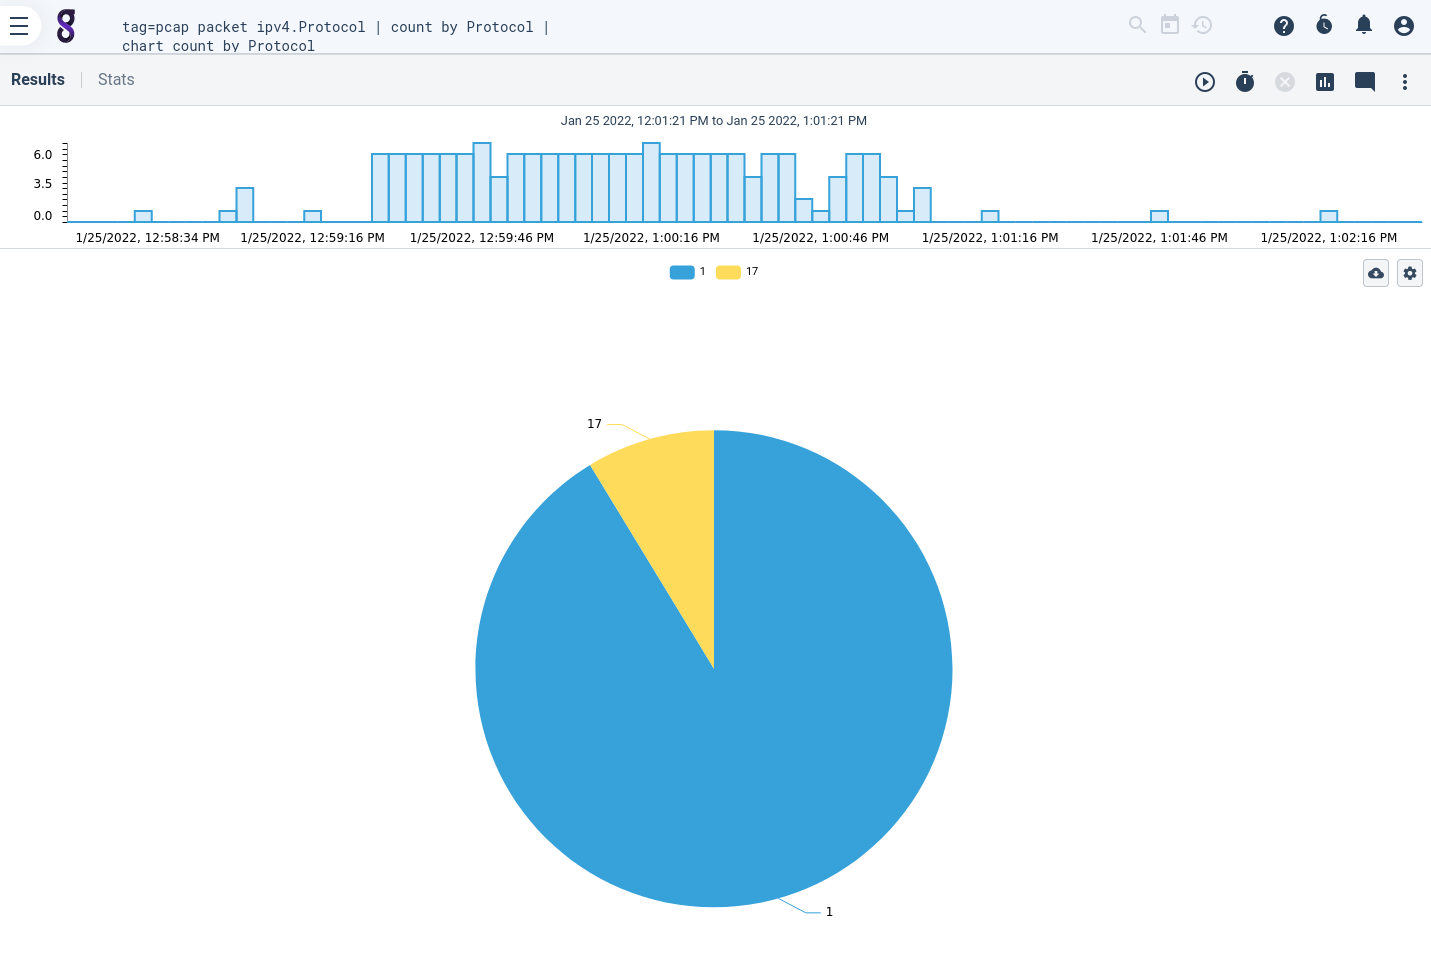
\includegraphics{images/igst-pcap-lab3.png}
	\caption{Protocol Ratios}
	\label{fig:pcap-lab3}
\end{figure}

To clean up after the experiment, simply run:

\code{docker kill \$(docker ps -a -q)}


\section{Tag Management / Federation}
\label{sec:federator}

The Federator is an entry relay: ingesters connect to the Federator and
send it entries, then the Federator passes those entries to an indexer.
The Federator can act as a trust boundary, securely relaying entries
across network segments without exposing ingest secrets or allowing
untrusted nodes to send data for disallowed tags. The Federator upstream
connections are configured like any other ingester, allowing
multiplexing, local caching, encryption, etc. Figure \ref{fig:federation}
shows an example architecture in which multiple Federators are used
to gather data from different business units into a central indexer pool.

\begin{figure}
	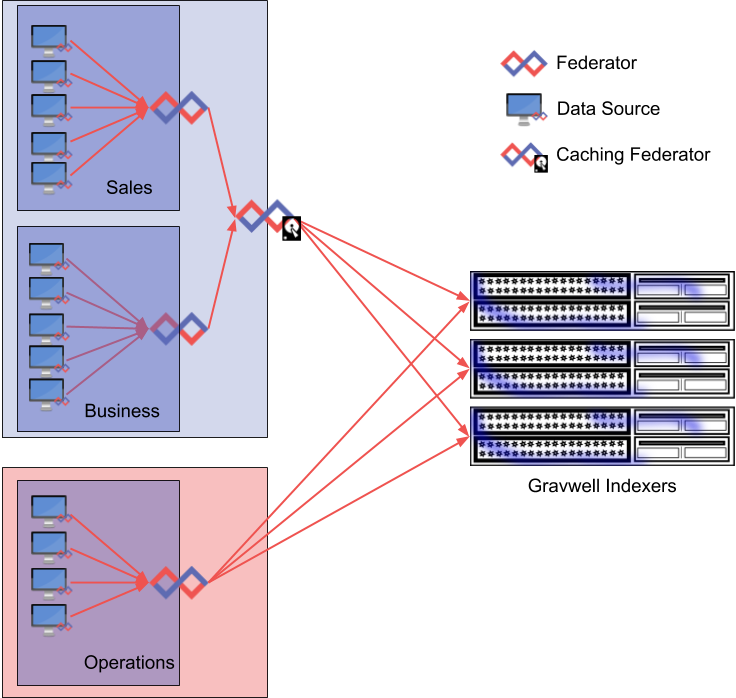
\includegraphics[width=0.75\linewidth]{images/federated-architecture.png}
	\caption{A Federated Architecture}
	\label{fig:federation}
\end{figure}

The Federator is well-suited for several use cases:

\begin{itemize}
\item
  Ingesting data across geographically diverse regions when there may
  not be robust connectivity
\item
  Providing an authentication barrier between network segments
\item
  Reducing the number of connections to an indexer
\item
  Controlling the tags and data source group can provide
\end{itemize}

The Federator can improve security by enforcing two kinds of controls:

\begin{itemize}
\item
  Auth: The Federator can use different Ingest Secrets on different
  listening ports. 
	\begin{itemize}
	\item Example: Assume two customers which will be uploading entries from ingesters in their own infrastructure to your indexer. By configuring a Federator with a separate listener and unique Ingest Secret for each customer, you can easily revoke one customer's access.
	\end{itemize}
\item
  Tags: The Federator can restrict which tags ingesters are allowed to
  use.
	\begin{itemize}
	\item Example: If multiple customers are uploading entries from their own ingesters, a Federator can ensure that Customer A only uploads entries tagged ``custA\_data'' and Customer B only uploads entries tagged ``custB\_data''.
	\end{itemize}
\end{itemize}

A sample configuration is shown below:

\begin{Verbatim}[breaklines=true]
[Global]
    Ingest-Secret = SuperSecretUpstreamIndexerSecret
    Connection-Timeout = 0
    Insecure-Skip-TLS-Verify = false
    Encrypted-Backend-target=172.20.232.105:4024
    Encrypted-Backend-target=172.20.232.106:4024
    Ingest-Cache-Path=/opt/gravwell/cache/federator.cache
    Max-Ingest-Cache=1024 #1GB
    Log-Level=INFO

[IngestListener "BusinessOps"]
        Ingest-Secret = CustomBusinessSecret
        Cleartext-Bind = 10.0.0.121:4023
        Tags=windows-*
        Tags=syslog

[IngestListener "DMZ"]
       Ingest-Secret = OtherRandomSecret
       TLS-Bind = 192.168.220.105:4024
       TLS-Certfile = /opt/gravwell/etc/cert.pem
       TLS-Keyfile = /opt/gravwell/etc/key.pem
       Tags=apache
       Tags=nginx
\end{Verbatim}

This configuration connects to two upstream indexers in a
\emph{protected} network segment and provides ingest services on two
\emph{untrusted} network segments. Each untrusted ingest point has a unique
\code{Ingest-Secret}, with one serving TLS with a specific certificate and
key pair. The configuration file also enables a local cache, making the
Federator act as a fault-tolerant buffer between the Gravwell indexers
and the untrusted network segments.

\subsection{Wildcard Tags}

When specifying an \code{IngestListener}, you may wish to accept a wide range of tags instead of just a handful of specific ones. Perhaps you're receiving Windows event logs from hundreds of different machines, and each one includes its hostname in the tag, e.g. ``winlog-activedirectory01''. The \code{Tags} field can contain wildcards, so you could match the example given by simply saying \code{Tags=winlog-*}.

\subsection{Hands-on Lab: Federation}

In this lab, we will configure a Federator with tag restrictions, then
attempt to send it entries with both allowed and disallowed tags. First,
launch a Gravwell webserver+indexer container:

\begin{Verbatim}[breaklines=true]
docker run --rm --net gravnet -p 8080:80 -d --name gravwell gravwell:base
\end{Verbatim}

Log into the web GUI (\href{http://localhost:8080}{http://localhost:8080}) and keep it open.

Start another container running the Federator:

\begin{Verbatim}[breaklines=true]
docker run --rm --net gravnet --name federator -it \
-e GRAVWELL_CLEARTEXT_TARGETS=gravwell:4023 \
gravwell:ingesters /opt/gravwell/bin/gravwell_federator
\end{Verbatim}

The container we are using has two pre-configured listeners for the
Federator:

\begin{itemize}
\item
  \code{enclaveA}, which listens on port 4001, allows entries tagged
  ``testA'', and uses the Ingest Secret ``enclaveASecrets''
\item
  \code{enclaveB}, which listens on port 4002, allows entries tagged
  ``testB'', and uses the Ingest Secret ``enclaveBSecrets''
\end{itemize}

With the Federator up and running, we use the generators container to attempt to send some JSON-formatted
entries to the Federator. We direct it to connect to the ``federator'' container on port 4001 and
use the secret ``enclaveASecrets'', which is the correct configuration
for the first IngestListener defined in the Federator config. However, note that we
add the option \code{-tag-name json}. This is not one of the allowed tags!

\begin{Verbatim}[breaklines=true]
docker run --net gravnet --rm -it gravwell:generators \
/jsonGenerator -clear-conns federator:4001 \
-ingest-secret enclaveASecrets -tag-name json
\end{Verbatim}

The command should fail, with an error message saying it
failed to negotiate tags:

\begin{Verbatim}[breaklines=true]
2020/02/05 18:44:25 ERROR: Timed out waiting for active connection due to All connections failed Failed to negotiate tags
\end{Verbatim}

This is expected, because we attempted to send entries tagged ``json'', which is not allowed! Let's run the generator again, this time specifying the allowed ``testA'' tag:

\begin{Verbatim}[breaklines=true]
docker run --net gravnet --rm -it gravwell:generators \
/jsonGenerator -clear-conns federator:4001 \
-ingest-secret enclaveASecrets -tag-name testA
\end{Verbatim}

We can verify that the entries made it in by running the query \code{tag=testA} in the Gravwell interface, as shown in Figure \ref{fig:federator-lab-1}.

\begin{figure}[H]
	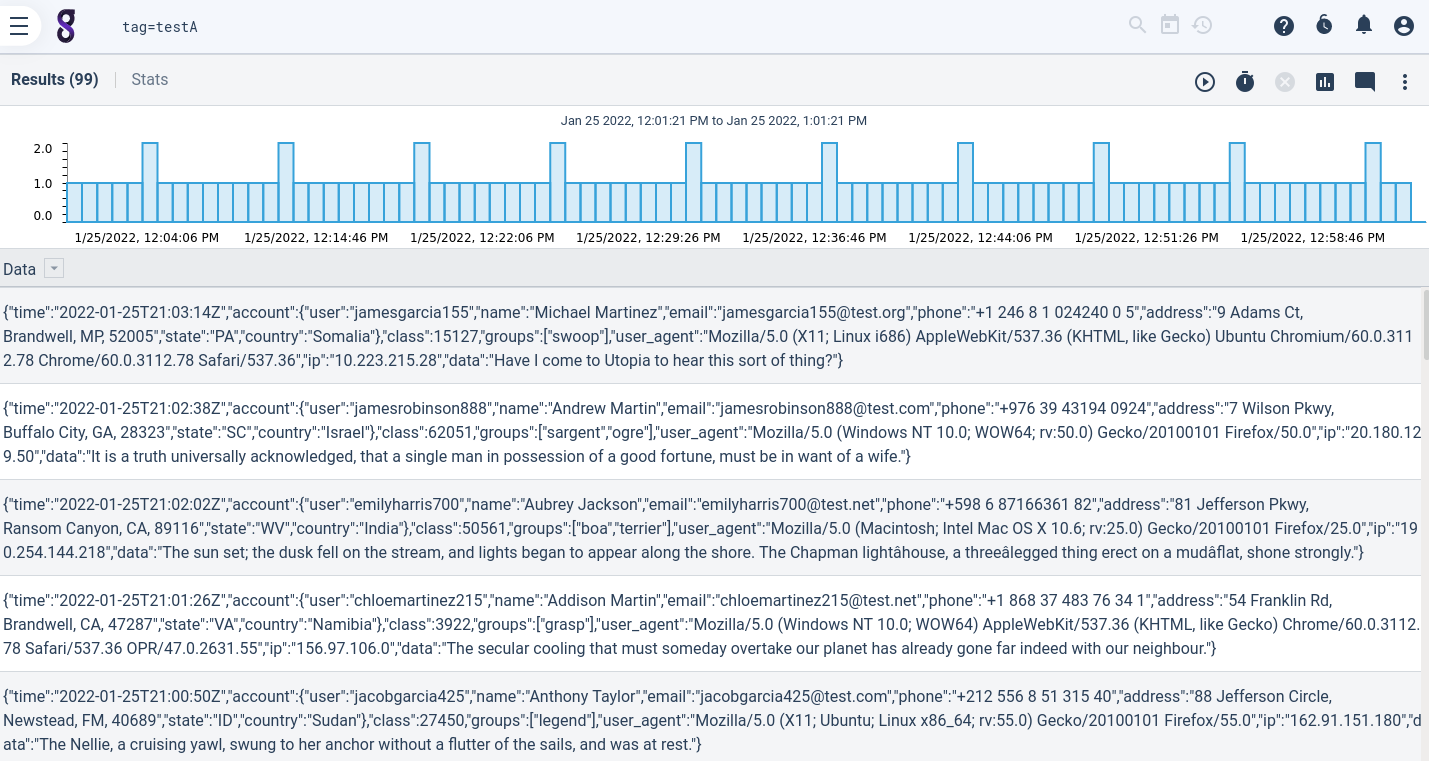
\includegraphics{images/igst-federator-lab.png}
	\caption{Entries Ingested via Federator}
	\label{fig:federator-lab-1}
\end{figure}

We can send entries to the other Federator listener by tweaking the generator command line, specifying port 4002, the secret ``enclaveBSecrets'', and tag ``testB'':

\begin{Verbatim}[breaklines=true]
docker run --net gravnet --rm -it gravwell:generators \
/jsonGenerator -clear-conns federator:4002 \
-ingest-secret enclaveBSecrets -tag-name testB
\end{Verbatim}

\section{Ingester Caching}

Ingester caching allows Gravwell ingesters to continue receiving data
and generating entries even when there are no active connections to
indexers. Entries are stored in an on-disk cache until indexer
communication is reestablished, at which point they are uploaded to the
indexer.

All officially-supported ingesters support caching. Caching is
controlled by two configuration options in the \code{[Global]} section of
the ingester configuration file:

\begin{itemize}
\item
  \code{Ingest-Cache-Path}: specifies the full path of the file which should
  be used for the cache, e.g.
  \code{/opt/gravwell/cache/file\_follow.cache}. Setting this option to a
  non-empty string enables ingester caching. If the specified file does
  not exist, a new one will be created.
\item
  \code{Max-Ingest-Cache}: specifies a maximum size (in megabytes) for the
  cache file. Once the cache has reached this size, later entries may be
  dropped.
\end{itemize}

The ingest cache is suitable for use with all ingesters except the File
Follower. Gravwell recommends against using a cache with the File
Follower ingester because the on-disk source files essentially
constitute their own cache. The Federator is especially useful when
caching is enabled; it can provide an extra level of resilience between
the ingesters and the indexers, allowing ingesters to push their entries
to the Federator even when the indexer is unavailable.

\subsection{Hands-on Lab: Ingester Cache}

In this lab we will stand up a Simple Relay ingester with cache enabled
and send it traffic while the Gravwell indexer is unavailable. First,
launch a Gravwell webserver+indexer container:

\begin{Verbatim}[breaklines=true]
docker run --rm --net gravnet -p 8080:80 -d --name gravwell gravwell:base
\end{Verbatim}

Log into the web GUI (\href{http://localhost:8080}{http://localhost:8080}) and leave the page open.

Then make the ingester container:

\begin{Verbatim}[breaklines=true]
docker run --rm --net gravnet --name ingesters -d \
-e GRAVWELL_CLEARTEXT_TARGETS=gravwell \
gravwell:ingesters /opt/gravwell/bin/gravwell_simple_relay
\end{Verbatim}

The ingesters container ships with a default Simple Relay configuration
which listens for line-delimited entries on port 7777, shown below:

\begin{Verbatim}[breaklines=true]
[Global]
Log-Level=INFO

[Listener "default"]
    Bind-String="0.0.0.0:7777"
    Ignore-Timestamps=true
    Tag-Name=default
\end{Verbatim}

Copy the file out:

\begin{Verbatim}[breaklines=true]
docker cp ingesters:/opt/gravwell/etc/simple_relay.conf /tmp/simple_relay.conf
\end{Verbatim}

Edit \code{/tmp/simple\_relay.conf} and add the following line to the \code{[Global]} section:

\code{Ingest-Cache-Path=/opt/gravwell/cache/simple\_relay.cache}

Then copy the config file back in and restart the container:

\begin{Verbatim}[breaklines=true]
docker cp /tmp/simple_relay.conf ingesters:/opt/gravwell/etc/simple_relay.conf
docker restart ingesters
\end{Verbatim}

Now that the ingester is configured and running, we will pause the indexer container.
Run this command on the host:

\begin{Verbatim}[breaklines=true]
docker pause gravwell
\end{Verbatim}

Now we open a shell on the ingester container:

\begin{Verbatim}[breaklines=true]
docker exec -it ingesters /bin/sh
\end{Verbatim}

From the ingester container's shell prompt, we now use a loop to
send 200,000 entries to the ingester:

\begin{Verbatim}[breaklines=true]
for i in `seq 1 200000`
do
	echo this is an entry $i
done | nc -w 1 localhost 7777
\end{Verbatim}

{The cache file is always initialized to 4 MB, but after pushing so many
entries we can check and see that it has grown:}

\begin{Verbatim}[breaklines=true]
/ # ls -lh /opt/gravwell/cache
total 17M    
-rw-r-----    1 root     root       16.8M Mar 15 17:03 simple_relay.cache
\end{Verbatim}

To flush the cache, we simply unpause the container on the host side:

\begin{Verbatim}[breaklines=true]
docker unpause gravwell
\end{Verbatim}

And verify that the cache has been emptied within the ingester
container:

\begin{Verbatim}[breaklines=true]
/ # ls -lh /opt/gravwell/cache
total 24K    
-rw-r-----    1 root     root        4.0M Mar 15 17:05 simple_relay.cache
\end{Verbatim}

Execute a search on the default tag (\code{tag=default}) to verify
that the entries were properly ingested, as in Figure \ref{fig:cache-lab}

\begin{figure}
	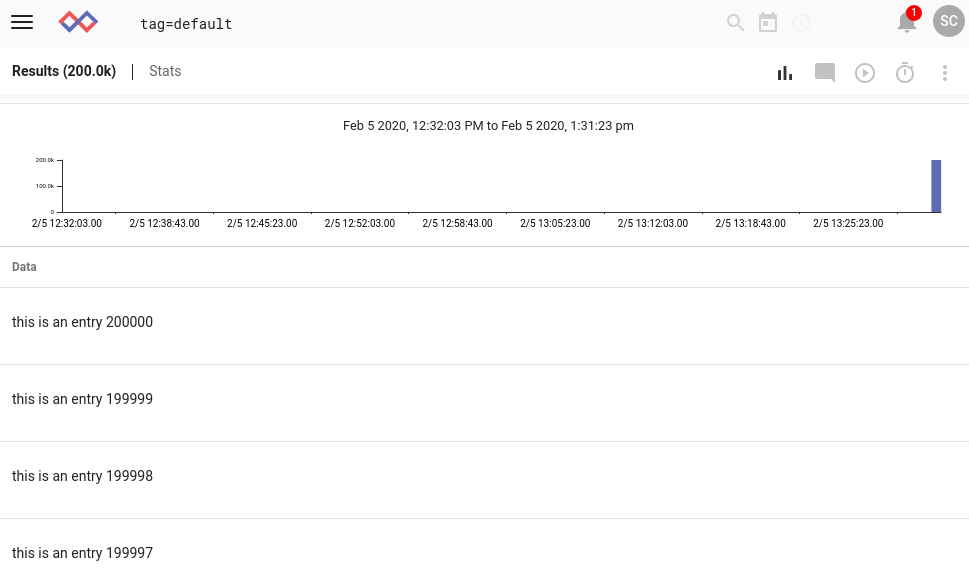
\includegraphics{images/igst-cache-lab.png}
	\caption{Previously-Cached Entries}
	\label{fig:cache-lab}
\end{figure}

To clean up after the experiment, simply run:

\code{docker kill \$(docker ps -a -q)}




\section{Ingest API and Source Code}

Gravwell's ingest library is open-sourced for public use at
\href{github.com/gravwell/gravwell/tree/master/ingest}{github.com/gravwell/gravwell/ingest}.
This makes it relatively easy to write a custom ingester for a specific
use case completely independent of Gravwell Inc. The open-source
ingesters found at
\href{github.com/gravwell/gravwell/tree/master/ingesters}{github.com/gravwell/gravwell/ingesters} provide
useful examples of real-world ingesters, but for the sake of
demonstration this document will describe the basic steps required to
ingest data, including code samples.

\subsection{Configuring and Starting the Ingest Muxer}

The Ingest Muxer is the standard way to connect to one or more Gravwell
indexers. If multiple indexers are specified, it will multiplex incoming
entries across all indexers evenly, hence the name. To instantiate a
muxer, define a UniformMuxerConfig:

\begin{Verbatim}[breaklines=true]
targets := []string{ "tcp://10.0.0.1:4023", "tcp://10.0.0.2:4023"}
secret := "IngestSecrets"
tags := []string{ "default" }
ingestConfig := ingest.UniformMuxerConfig{
    Destinations: targets,
    Tags:         tags,
    Auth:         secret,
}
\end{Verbatim}

There are three essential arguments in the muxer config:

\begin{itemize}
\item
  \code{Destinations}: a list of strings describing how to connect to an
  indexer, e.g. ``tcp://10.0.0.1:4023''.
\item
  \code{Tags}: a list of strings containing the tags the ingester will use
\item
  \code{Auth}: a string containing the shared secret used to authenticate with
  the indexers.
\end{itemize}

With the UniformMuxerConfig defined, instantiate and start the muxer:

\begin{Verbatim}[breaklines=true]
    igst, err := ingest.NewUniformMuxer(ingestConfig)
    if err != nil {
        log.Fatalf("Failed build our ingest system: %v\n", err)
    }
    defer igst.Close()
    if err := igst.Start(); err != nil {
        log.Fatalf("Failed start our ingest system: %v\n", err)
    }
\end{Verbatim}


After calling \code{Start()} on the muxer, one should typically call
\code{WaitForHot} to wait until at least one indexer connection is live.
The argument to \code{WaitForHot} is a timeout in case no indexer
connections are established:

\begin{Verbatim}[breaklines=true]
    if err := igst.WaitForHot(60 * time.Second); err != nil {
        log.Fatalf("Timedout waiting for backend connections: %v\n", err)
    }
\end{Verbatim}


\subsection{Creating and Uploading Entries}

Once the muxer has been started and \code{WaitForHot} has returned
successfully, entries can be sent to the indexer(s). Note, however, that
indexers use a mapping of string tag names to numeric tag IDs, and that
entries sent to the indexer must use the \code{numeric} tag IDs, not string
tags. Thus, we first query the ingest muxer for the tag ID of the
``default'' tag:

\begin{Verbatim}[breaklines=true]
    defaultTagID, err := igst.GetTag("default")
    if err != nil {
        log.Fatalf("Failed to get tag: %v", err)
    }
\end{Verbatim}

Having acquired the tag, we are now able to build an Entry:

\begin{Verbatim}[breaklines=true]
    ent := entry.Entry{
        TS:   entry.Now(),
        SRC:  net.ParseIP("127.0.0.1"),
        Tag:  defaultTagID,
        Data: []byte("This is my test data!"),
    }

\end{Verbatim}


The components of an Entry are:

\begin{itemize}
\item
  \code{TS} The timestamp attached to the entry. Although this example uses
  the current time, it can be set to anything. The timestamp should generally indicate when
  the \emph{data} was generated, not when the \emph{entry} was created.
\item
  \code{SRC}: An IP address to represent the source of the data. We are using
  127.0.0.1 for this example, but any IPv4 or IPv6 address is valid.
\item
  \code{Tag}: A numeric tag ID as derived from the \code{GetTag} function.
\item
  \code{Data}: A slice of bytes that makes up the actual \emph{content} of the
  entry. This can be literally anything.
\end{itemize}

With the Entry built, the only thing remaining is to send it to the
indexer:

\begin{Verbatim}[breaklines=true]
    if err := igst.WriteEntry(&ent); err != nil {
        log.Fatalf("Failed to write entry: %v", err)
    }
\end{Verbatim}

\subsection{Cleaning Up/Shutting Down}

An ingester will typically start up, build its muxer, and then go into
a loop building and uploading Entries until it either runs out of data
or receives a signal from the operating system that it should shut down.
In order to shut down nicely, call the \code{Sync} and \code{Close} functions on the
muxer:

\begin{Verbatim}[breaklines=true]
if err := igst.Sync(time.Second); err != nil {
    log.Fatalf("Failed to sync: %v\n", err)
}
igst.Close()
\end{Verbatim}



\section{Permissions and Port Binding}

Gravwell is designed to execute with as few privileges as possible.
The shell and Debian installers will create an unprivileged user and
group named gravwell and create a directory structure in
\code{/opt/gravwell} which is owned by the gravwell user.
Most of the services don't need any special privileges, however
if we want to be able to serve the Gravwell GUI on traditional HTTP and
HTTPS ports we will need the ability to bind to port 80 and port 443,
which are privileged system ports. Modern Linux kernels have the
ability to assign
capabilities\footnote{http://man7.org/linux/man-pages/man7/capabilities.7.html} to
executables. Capabilities grant specific privileges that would normally be 
denied to the executing user. Gravwell uses these capabilities to enable the
webserver to bind to privileged ports without requiring that we execute
as an elevated user or group.

When debugging broken Gravwell installations there are a few things to
always check:

\begin{enumerate}
\item
  The ownership of files in \code{/opt/gravwell} and any well locations. They should be owned by \code{gravwell:gravwell}
\item
  The capabilities assigned to binary files.
	\begin{enumerate}
	\item
	  The webserver needs CAP\_NET\_BIND\_SERVICE
	\item
	  The network capture ingester needs CAP\_NET\_RAW
	\end{enumerate}
\item
  Check logs for critical error messages.
	\begin{enumerate}
	\item \code{/opt/gravwell/log}
	\item \code{/opt/gravwell/log/web}
	\item \code{/opt/gravwell/log/crash}
	\item \code{/dev/shm/}
	\end{enumerate}
\end{enumerate}

The most common breakages are when users move shards or attempt to
manually start a Gravwell component as \code{root}; this causes Gravwell to
assign ownership of files and directories to the root user and
group. When Gravwell is then started correctly by systemd, the Gravwell
processes (running as the \code{gravwell} user) won't have access to the
files and folders they need.

\subsection{Hands-on Lab: Permissions and Port Binding}

Docker typically just executes everything as root, so we will be using
a new container that actually uses a proper user and group to execute
Gravwell components. Start by cleaning up the environment:

\code{docker kill \$(docker ps -q)}

Ensure the \code{gravwell:brokenperms} container is loaded (if you don't have the \code{gravwell:brokenperms} image, see Section \ref{sec:load-lab-images} for instructions on how to load it), then start it:

\begin{Verbatim}[breaklines=true]
docker run -d --net gravnet -p 8080:80 --rm \
--name test gravwell:brokenperms
\end{Verbatim}

Check the GUI (\href{http://localhost:8080}{http://localhost:8080}), are we able to access Gravwell? Is the container up?

Let's grab a shell within the container as the root user and start
poking around:

\begin{Verbatim}[breaklines=true]
docker exec -it --user root test /bin/bash
\end{Verbatim}

The goal is to fix the installation and get the Gravwell components to
start correctly. Start by answering a few questions:

\begin{enumerate}
\item
  Which services are not starting?
\item
  Where are the pertinent log files?
\item
  What other locations contain Gravwell logs?
\item
  What are the permissions inside \code{/opt/gravwell/}?
	\begin{enumerate}
	\item
	  What should they be?
	\end{enumerate}
\item
  What are the capabilities assigned to each Gravwell service binary?
	\begin{enumerate}
	\item
	  What should they be?
	\end{enumerate}
\end{enumerate}

To clean up after the experiment, simply run:

\begin{Verbatim}[breaklines=true]
docker kill $(docker ps -a -q)
\end{Verbatim}



\section{Gravwell and Systemd}

{Gravwell installers assume the availability of Systemd. While there are
other init services out there, Systemd has steadily become the
init system of choice for most popular Linux distributions. Systemd
controls how processes start, how failures are handled, and how to
shutdown processes using unit
files\footnote{https://access.redhat.com/documentation/en-us/red\_hat\_enterprise\_linux/7/html/system\_administrators\_guide/sect-managing\_services\_with\_systemd-unit\_files}\footnote{https://www.digitalocean.com/community/tutorials/understanding-systemd-units-and-unit-files}.
Unit files can be installed in several locations, but Gravwell places
its unit files in \code{/etc/systemd/system/}. The unit files are copied
to the target folder, then registered and started using \code{systemctl
enable \textless{}service name\textgreater{}} and \code{systemctl start
\textless{}service name\textgreater{}}.

This is the unit file for the Gravwell indexer that is shipped for
version 3.3.5:

\begin{Verbatim}[breaklines=true]
[Install]
WantedBy=multi-user.target

[Unit]
Description=Gravwell Indexer Service
After=network-online.target
OnFailure=gravwell_crash_report@%n.service

[Service]
Type=simple
ExecStart=/opt/gravwell/bin/gravwell_indexer -stderr %n
ExecStopPost=/opt/gravwell/bin/gravwell_crash_report -exit-check %n
WorkingDirectory=/opt/gravwell
Restart=always
User=gravwell
Group=gravwell
StandardOutput=null
StandardError=journal
LimitNPROC=infinity
LimitNOFILE=infinity
TimeoutStopSec=120
KillMode=process
KillSignal=SIGINT
\end{Verbatim}

By default we do not limit the number of files or processes that
Gravwell has access to. Large systems can spread out and run many
threads and while managing potentially thousands of shards. However, if
your Gravwell is co-resident with other important services it may be
desirable to limit access to resources. We do not recommend limiting
the number of open files or processes, but limiting CPU access and
memory usage may be desirable. CPU and memory can be limited using the
\code{CPUQuota} and \code{MemoryMax} parameters in the
\code{[Service]} block. IO and network resources can also be limited
using
\code{IO}\footnote{https://www.freedesktop.org/software/systemd/man/systemd.resource-control.html}.


\section{Gravwell and Docker}

Gravwell supports Docker as a first class citizen (as you can tell by
our heavy use for this training). Most components can use environment
variables and Docker secrets for configuration and process control. Our
published Docker container uses a process control daemon called
manager\footnote{https://github.com/gravwell/manager} which
can monitor environment variables that tell it to disable services. The
available control parameters are fully documented in
Gravwell's web documentation\footnote{https://docs.gravwell.io/\#!configuration/docker.md},
but let's dive into controlling Gravwell processes and control
parameters using docker.

Gravwell services have a hierarchy of configuration sources when
starting. Configuration parameters in a configuration file are checked
first; if a mandatory configuration parameter is empty, it will then
potentially look for the configuration parameter in an environment
variable. The environment variable is a two step lookup. First it
checks if an environment variable is set indicating that we should use
secrets. Docker secrets are only available when operating in swarm
mode\footnote{https://docs.docker.com/engine/swarm/secrets/}.
Kubernetes\footnote{https://kubernetes.io/docs/concepts/configuration/secret/} and
OpenShift\footnote{https://docs.openshift.com/container-platform/3.5/dev\_guide/secrets.html} have
similar systems that are compatible with Docker secrets and thus
Gravwell. Rather than attempt to get a full Docker swarm environment
up, configuration parameters can also be set as regular Docker
environment variables. The core Gravwell package supports the following
environment/secret configuration parameters:

\begin{Verbatim}[breaklines=true]
GRAVWELL_REMOTE_INDEXERS
GRAVWELL_REPLICATION_PEERS
GRAVWELL_INDEXER_UUID
GRAVWELL_WEBSERVER_UUID
GRAVWELL_INGEST_AUTH
GRAVWELL_CONTROL_AUTH
GRAVWELL_SEARCHAGENT_AUTH
GRAVWELL_DATASTORE
GRAVWELL_DATASTORE_LISTEN_ADDRESS
GRAVWELL_DATASTORE_LISTEN_PORT
\end{Verbatim}

If \code{GRAVWELL\_ENABLE\_DOCKER\_SECRETS} is set to TRUE, then Gravwell
will attempt to load the configuration parameters from the secrets
system, otherwise it looks for the value in an environment variable. We
use the environment variable method of configuration extensively
throughout this training. Run \code{docker inspect gravwell:base} and
examine the \code{Config} and \code{Env} sections. Those environment
variables can be overridden when building a container using
the \code{-e} flag. For example, \code{docker run -d -\/-name test -e
GRAVWELL\_INDEXER\_UUID=611757dc-4b54-11e9-acf8-aba211cc704f
gravwell:base} will start the indexer with a specific UUID, preventing
it from generating and assigning a random value.

\subsection{Hands-on Lab: Gravwell and Docker}

For this lab we will examine how to use Docker to modify core
configuration variables at runtime while deploying a base
\code{gravwell.conf} file. To start, let's clean the working environment:

\code{docker kill \$(docker ps -q)}

Now create a new container named test using the gravwell:base image.
When you create the container, override the default \code{Ingest-Auth},
\code{Control-Auth}, and \code{Search-Agent-Auth} auth tokens with something
unique. Once the container has been created using \code{docker create},
log into the GUI and check that
everything came up, then try ingesting some data using JSON generator; be sure to
set the appropriate authentication secrets!

\begin{Verbatim}[breaklines=true]
docker run --net gravnet --rm -it gravwell:generators \
/jsonGenerator -clear-conns test \
-ingest-secret MY_SECRET
\end{Verbatim}

\subsubsection{Lab Questions}

\begin{enumerate}
\item
  How can we check the environment variable overrides using Docker?
\item
  Why is it insecure to use environment variables to configure
  authentication tokens?
\item
  Why is this configuration system essential for deployment using
  something like Kubernetes or OpenShift?
\end{enumerate}
